\documentclass[a4paper,12pt,titlepage]{article}
\usepackage{verbatim}
\newcommand{\HRule}{\rule{\linewidth}{0.5mm}}
\usepackage{float}
\usepackage{graphicx}
\usepackage[utf8]{inputenc}
\usepackage{hyperref}
\usepackage{minitoc}
\usepackage{minted}

\DeclareGraphicsExtensions{.PNG,.png,.jpg,.JPG}
\graphicspath{{./Images/}}
%\end{comment}

\begin{document}



\begin{titlepage}
\begin{center}

\includegraphics[width = 0.3\textwidth]{US_logo.png}~\\[1cm]
\textsc{\LARGE Unsolvable Solutions}\\
Client: Francois Mouton at the CSIR DSSR\\[1.5cm]
\textsc{\Large  User Manual}\\[0.5cm]

 \HRule\\[0.4cm]
{ \huge \bfseries  Eavesdropping Protection in Conclave \\[0.4cm] }

 \HRule\\ 



Github link:  \url{https://github.com/Unsolvable-Solutions/Project-EPIC} \\[1.2cm]

\noindent
\begin{minipage}[t]{0.4\textwidth}

	\begin{flushleft} \large
	\emph{Members:}\\
		Edwin Fullard  \\
		Jaco Bezuidenhoudt \\
		Jandre Coetzee\\
		Maret Stoffberg\\
		Ryno Pierce\\
	\end{flushleft}
\end{minipage}%
\begin{minipage}[t]{0.4\textwidth}
\begin{flushright} \large
	\emph{Student Number:} \\
		12048675 \\
		11013878 \\
		 10693077 \\
		 11071762 \\
		 12003922\\
	\end{flushright}
\end{minipage}

\vfill


% Bottom of the page




\end{center}
\end{titlepage}

\tableofcontents


\newpage
\section{System Overview}
The purpose of the EPIC(Eavesdropping protection in Conclave) project is to protect the confidential information discussed in a meeting. This is achieved by making sure the users phone or tablets data, wifi and GSM are switched off during the meeting.

This EPIC project consist of a server, Android application, NFC Node, Website, and an Intel Edison device. 
The Android device is held over the NFC Node. The NFC then sends a request to the server via the Edison to enter the meeting. The server then responds with access granted or not. If access is granted, the user may the proceed to the meeting and the data, wifi and GSM of the device is turned off. When the user then exists the meeting, the device is held over the Node again and the previous state of the phone is restored. 
The website is used to register, create a new meeting and to query the attendance log of any past meeting.

\newpage
\section{System Configuration}

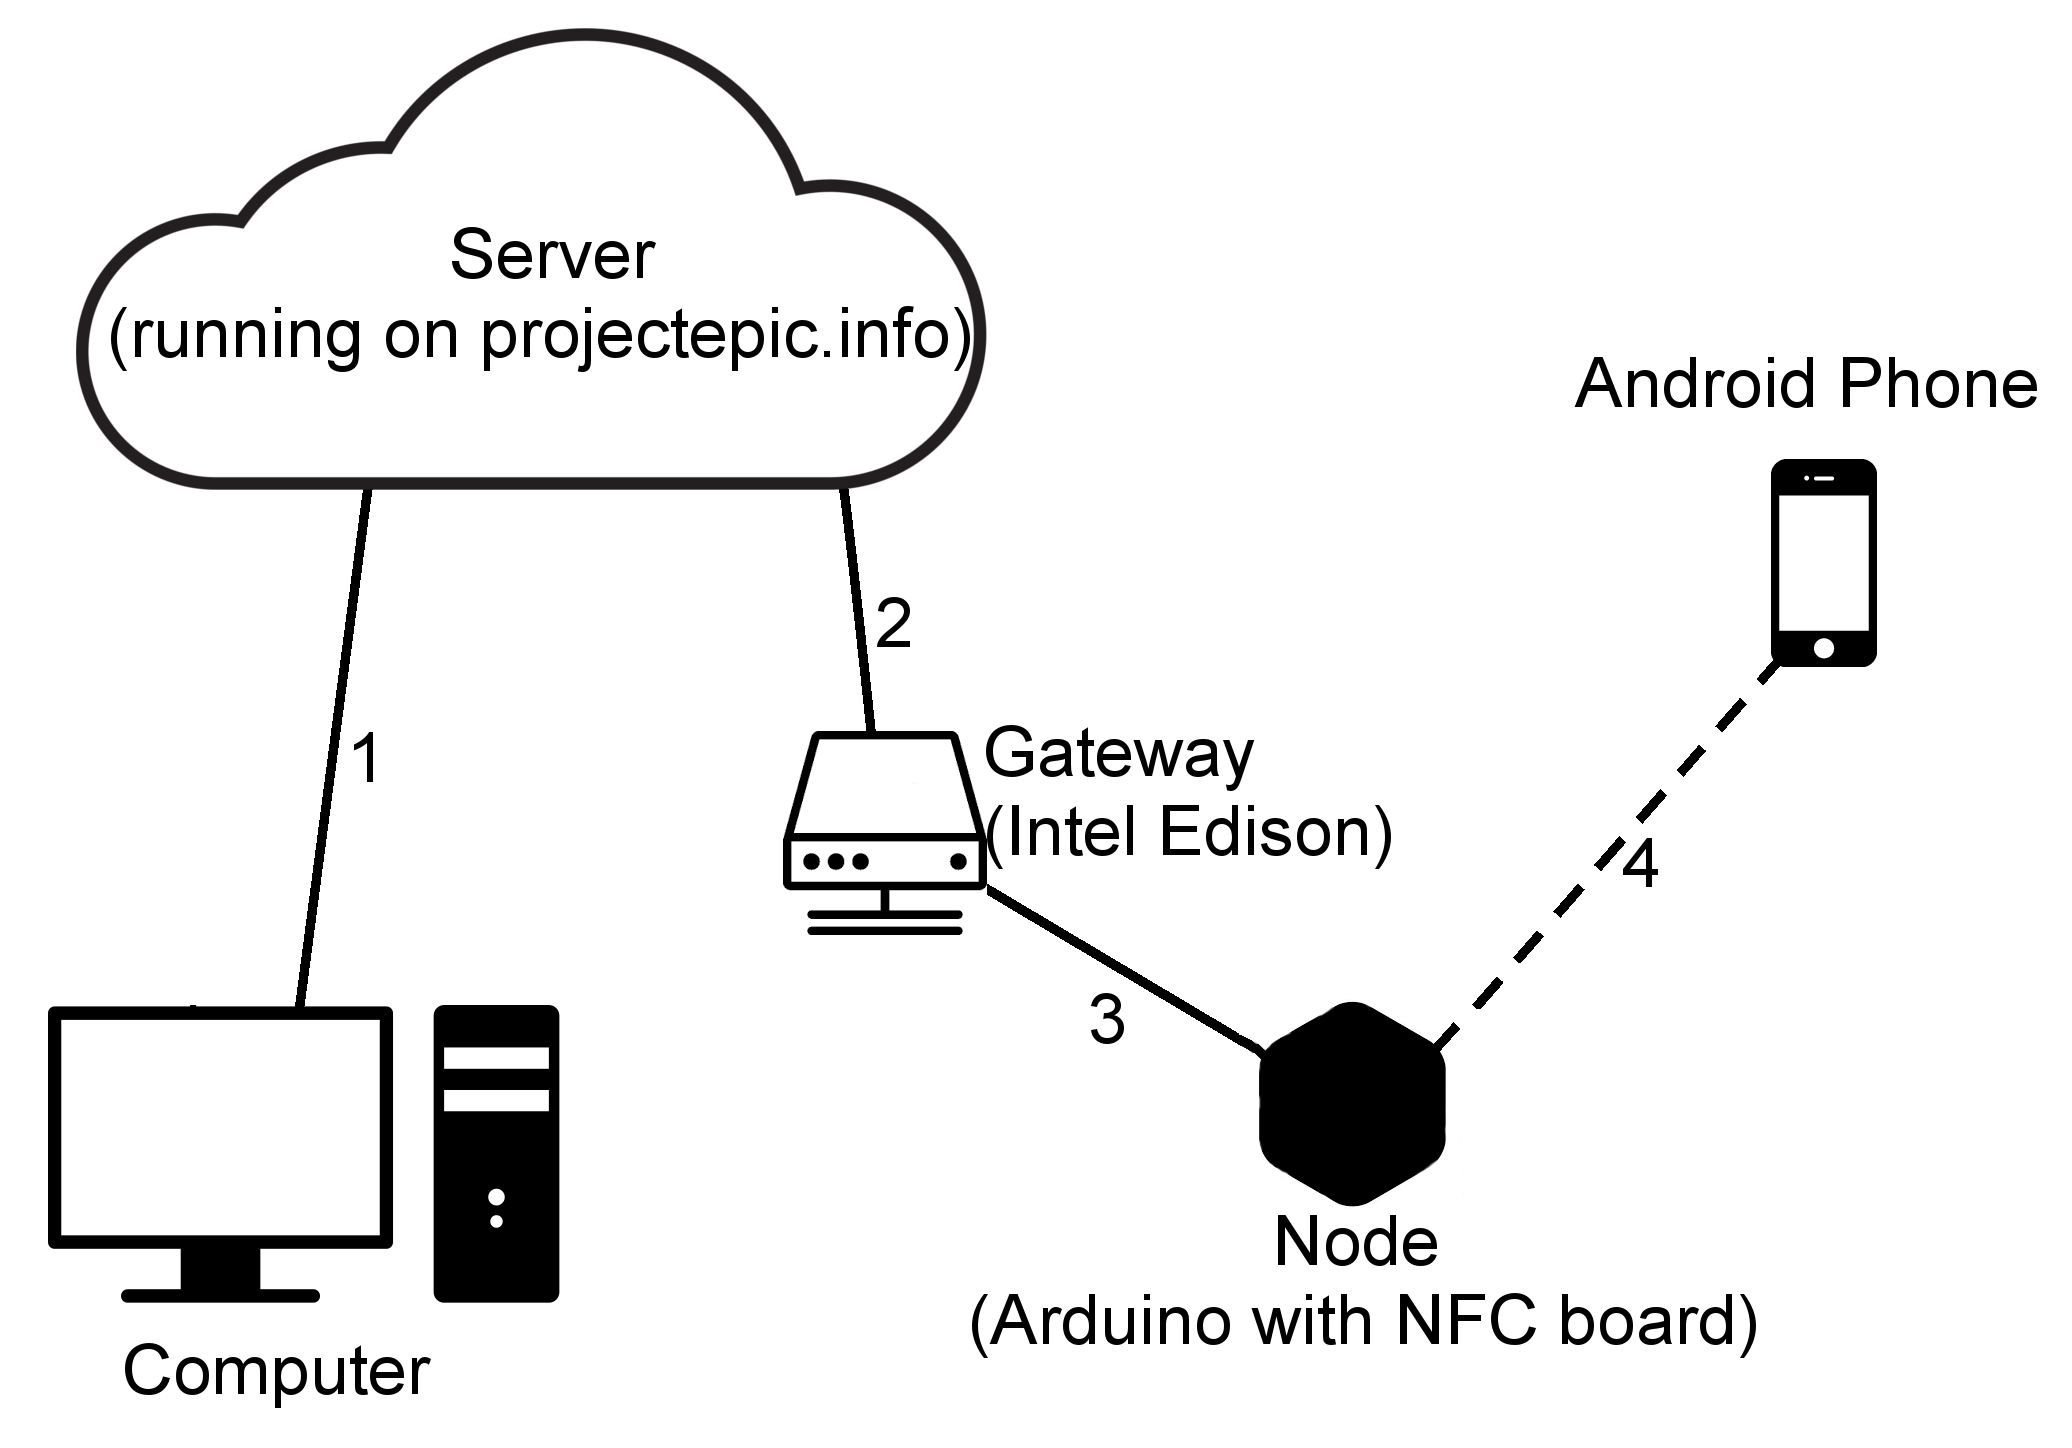
\includegraphics[width=12cm, height=8.5cm]{SystemLayout}
\begin{enumerate}
\item The website connects through the Internet via a web browser.
\item The Gateway connects to the server via wifi. It relays the data from the Node to the Server and vice versa.
\item The Gateway and Node is connected using a cable. It sends the users' information, obtained from the phone via NFC, to the Gateway, and transmits results  received from the Gateway, via NFC to the Phone.
\item The phone connects to the Node using NFC. The phone sends the users' email address, device identification and password, and then the Node sends back the response from the server to the phone.
\end{enumerate}



\newpage
\section{Installation}

\subsection{Android Application}
\begin{enumerate}
\item Copy the file name \textit{EPICApp.apk} over to your device. You can download the file from \url{https://github.com/Unsolvable-Solutions/Project-EPIC/tree/master/EPICProtectionApp/EPICAppFor4.4.2/app}.
\item Locate the file on your device and tap on the file.
\item A list of permissions will pop-up that the application needs in order to function. Click on the \textit{install} option.
\item The application is now ready to use.
\end{enumerate}

\subsection{Node}
\begin{enumerate}
\item Download the Arduino IDE for your respective OS. You can find it at\newline \url{https://www.arduino.cc/en/Main/Software}.
\item Download the source files from\newline \url{https://github.com/Unsolvable-Solutions/Project-EPIC/tree/master/EPICNode}.
\item Add all the libraries from the source file to the Arduino IDE.
\item Plug the Node into your computer and upload the source files through the Arduino IDE by following the steps provided in the Arduino IDE.
\end{enumerate}

\subsection{Intel Edison}
\begin{enumerate}
\item Download the Intel Edison Standalone driver. You can find it at\newline \url{https:// software.intel.com/en-us/iot/ hardware/edison/downloads}.
\item Attach the serial port at 115200 BAUD rate. This can be done in two ways.
\begin{itemize}
    \item For Windows: use \textit{PuTTY} as your serial terminal. You can find a clear guide  \href{https://software.intel.com/en-us/setting-up-serial-terminal-on-system-with-windows}{\textit{here}}.
    %at\newline \url{https://software.intel.com/en-us/setting-up-serial-terminal-on-system-with-windows}.
    \item For Linux: use \textit{Screen} as your serial terminal. You can find a clear guide 
     \href{https://software.intel.com/en-us/setting-up-serial-terminal-on-system-with-linux}{\textit{ here}}.
    % at \newline \url{https://software.intel.com/en-us/setting-up-serial-terminal-on-system-with-linux}.
\end{itemize}
\item Download (or clone) all the source files from \url{https://github.com/ Unsolvable-Solutions/ Project-EPIC/tree/master/EPICEdison}.
\item In your command line
\begin{itemize}
\item Redirect to the folder that you have just downloaded.
\item Run
\begin{minted}{python}
npm install
\end{minted}
\item Run 
\begin{minted}{python} 
npm start 
\end{minted}
\end{itemize}

\item The Intel Edison is now ready to use.
\end{enumerate}

\subsection{Server}
\begin{enumerate}
\item Install node and npm on your server. You can find a clear guide at  \url{https://docs.npmjs.com/getting-started/installing-node}
\item Download (or clone) all the source files from \url{https://github.com/Unsolvable-Solutions/Project-EPIC/tree/master/EPICServer}
\item Do the following in your command line to start the server
\begin{itemize}
\item Redirect to the folder that you have just downloaded.
\item Run
\begin{minted}{python}
npm install
\end{minted}
\item Run 
\begin{minted}{python} 
npm start 
\end{minted}
\end{itemize}
\item Make sure port 1337 is open in your firewall or that your webhost application point to \textit{localhost:1337}
\item Enjoy the server application
\end{enumerate}


\newpage
\section{Getting Started}

\subsection{Android Application}
\begin{enumerate}
\item To get started, first navigate to to application shortcut name EpicApp and open it.
\item If the NFC is turned off
\begin{itemize}
\item The following screen will be presented:
\begin{figure}[H]
\center
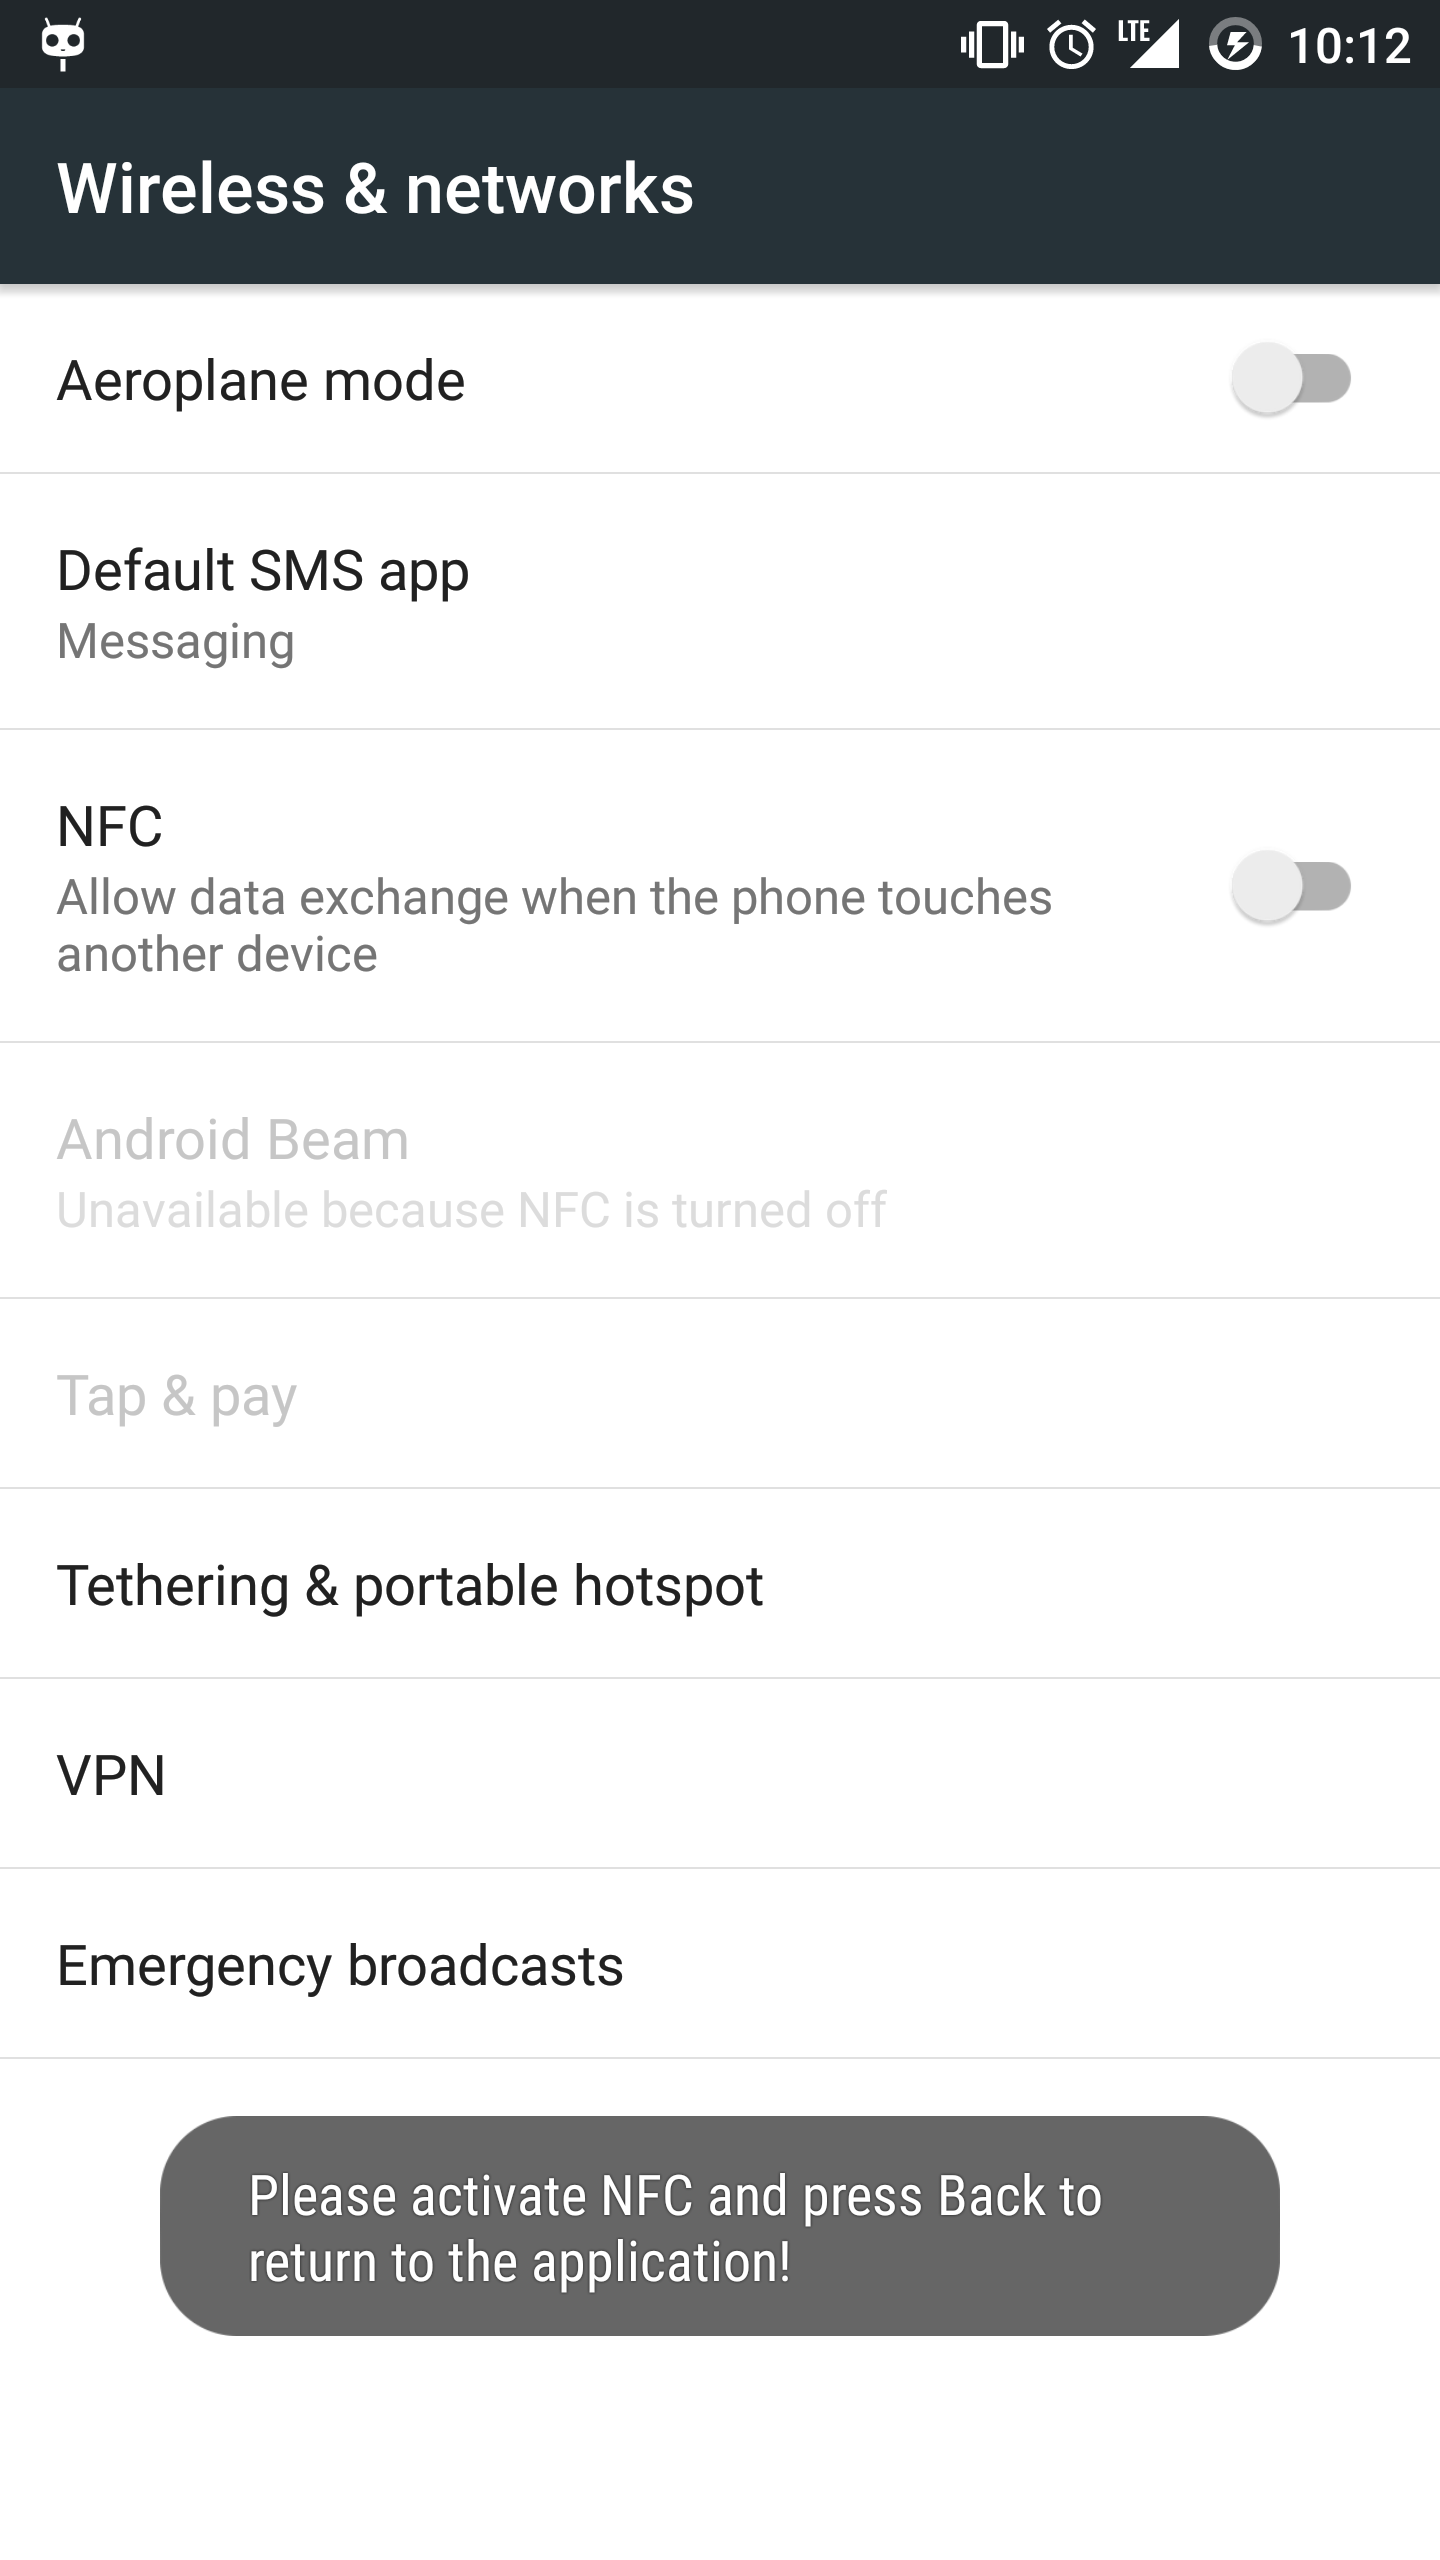
\includegraphics[height=6cm]{Settings}
\caption{NFC Settings}
\label{fig:my_label}
\end{figure}
\item Turn the NFC on by clicking on the slider.
\item After it is turned on, press the back button.
\end{itemize}

\item{ On the next screen there is an edit box with the text \textit{New Employee ID}. Click on it and type in the registered ID given to you and press the done or check mark key.
\begin{figure}[H]
\center
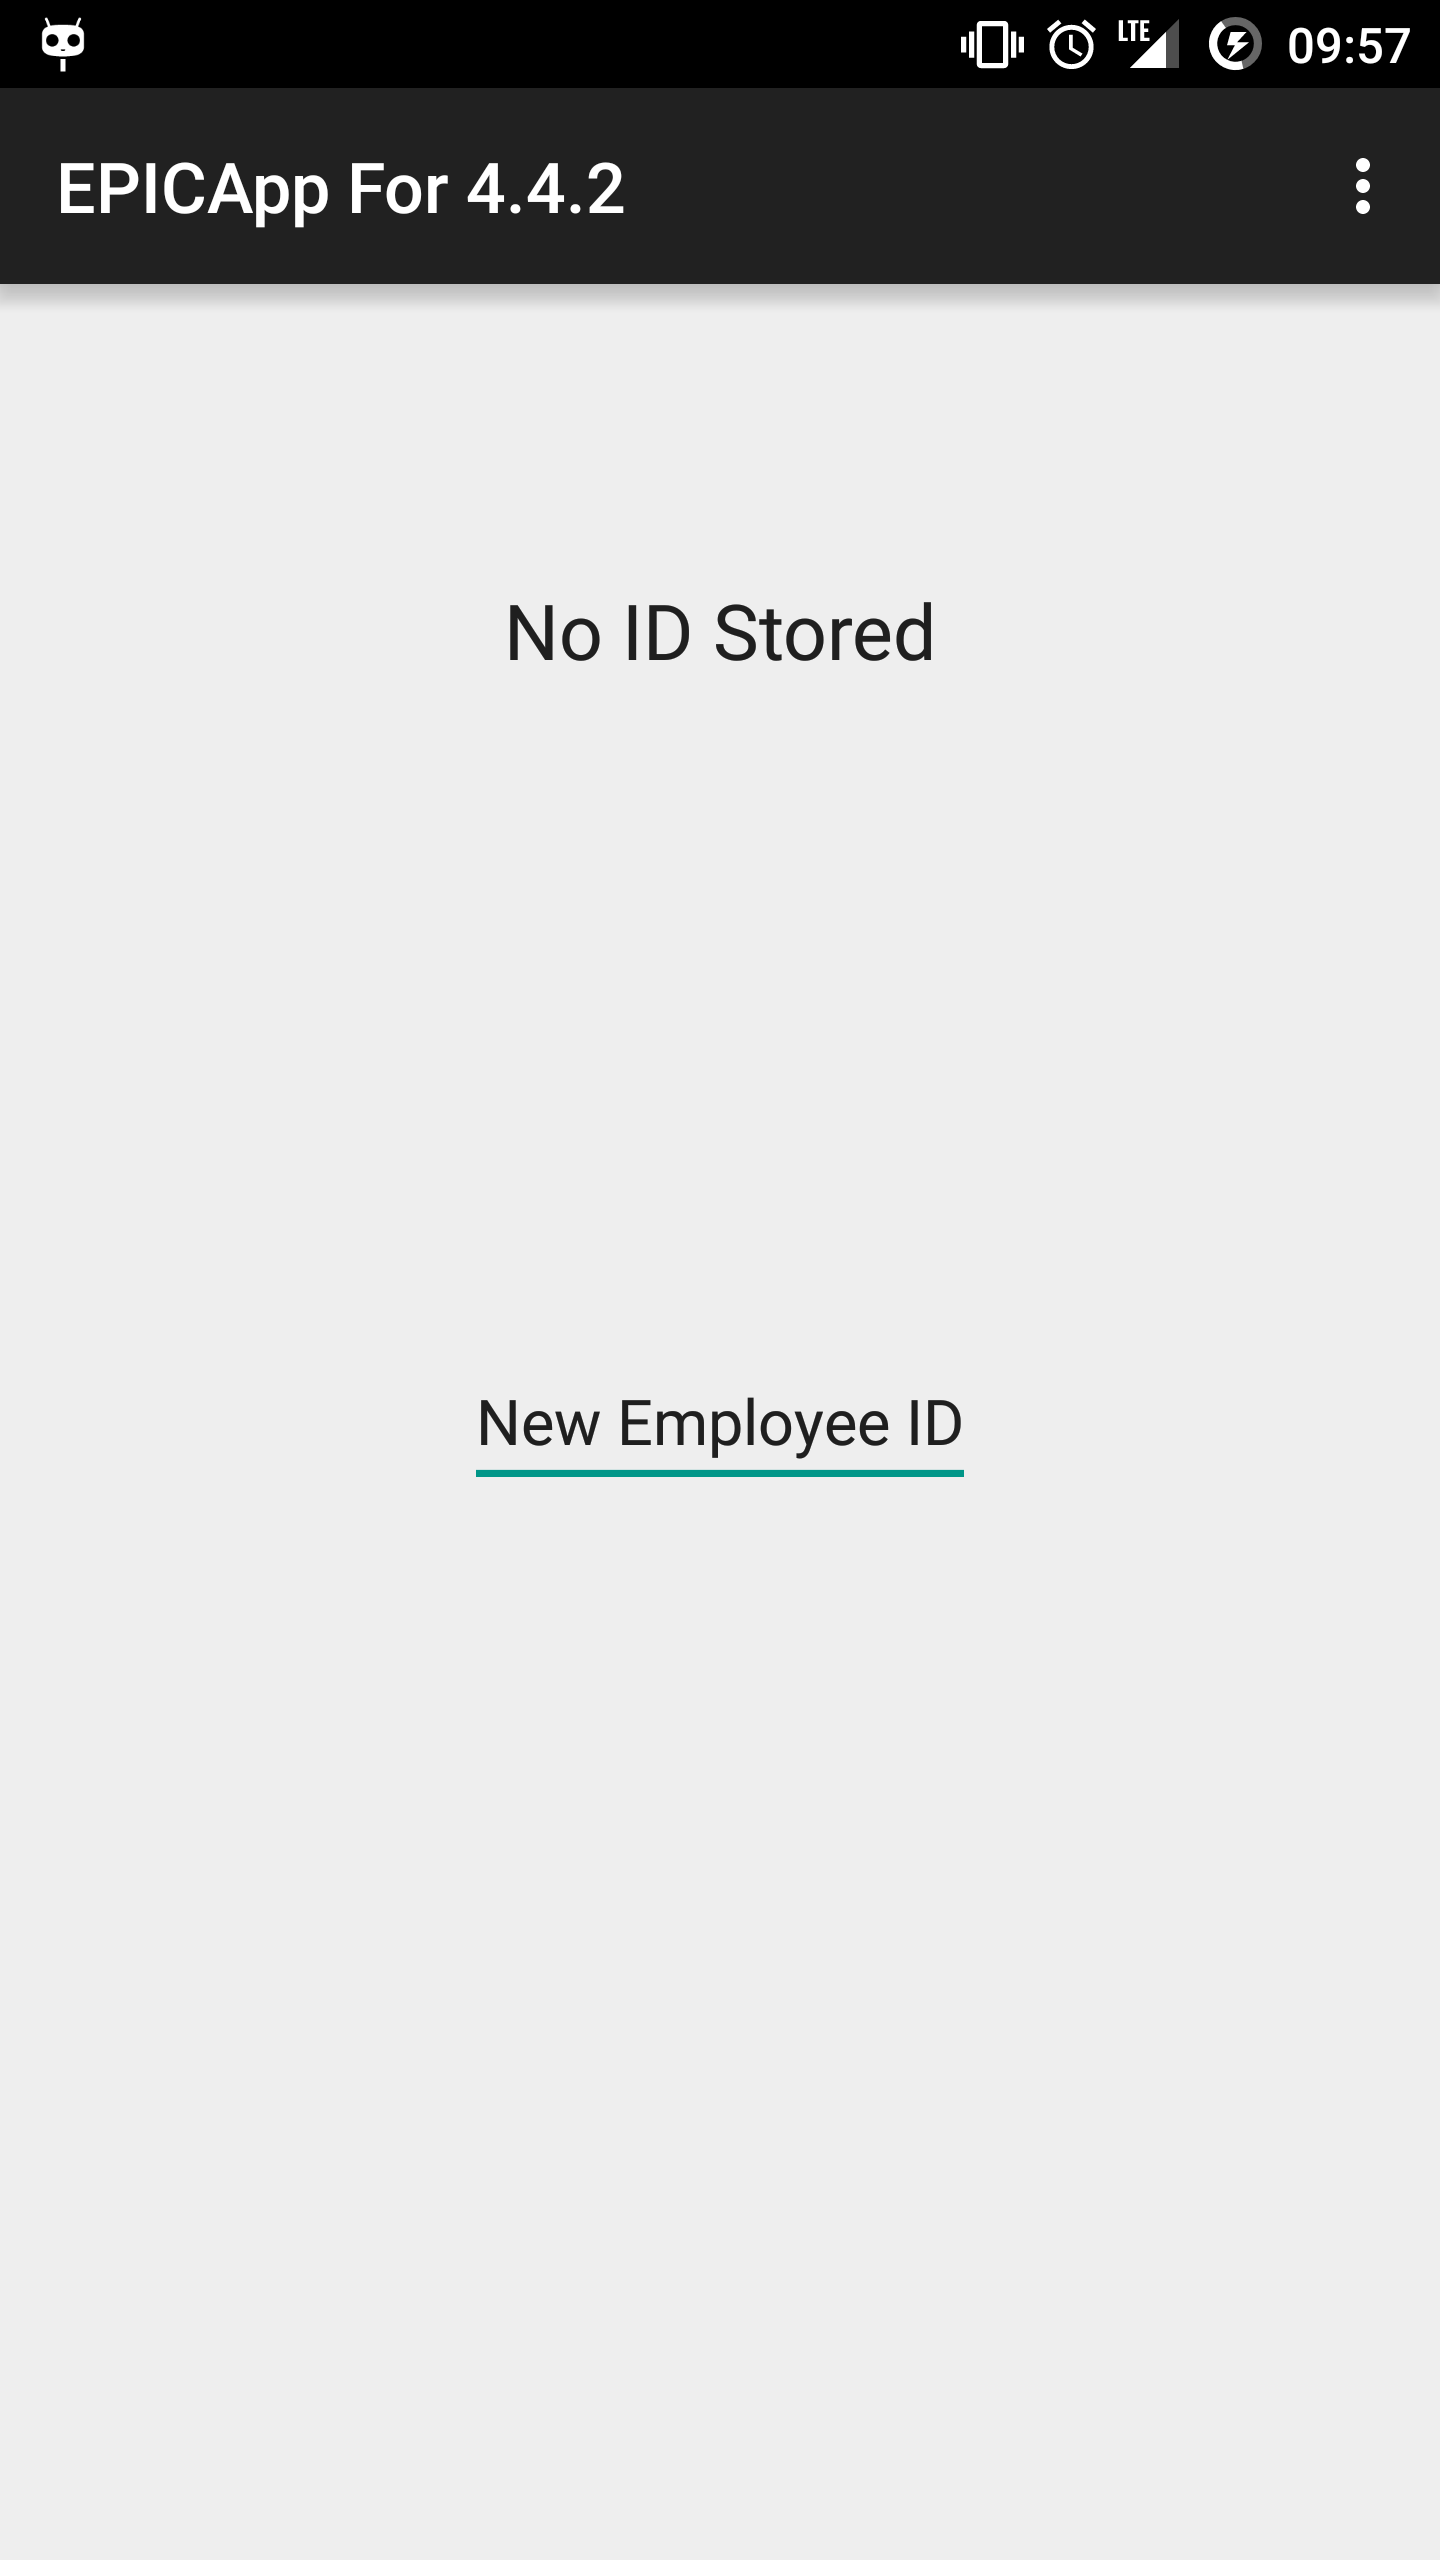
\includegraphics[height=6cm]{firstOpen}
\caption{Application's first use}
\label{fig:my_label2}
\end{figure}}
\item You will notice the \textit{No ID Stored} text change to your ID that you typed in. This means that the application is now ready to be used to enter the meeting room.
\end{enumerate}

\subsection{Node}
Connect the Node to the Gateway (Intel Edison) and check that the lights are Orange and Yellow strips running across.

\subsection{Website}
Open the website \url{projectepic.info} in your favourite browser.


\newpage
\section{Using The System}

\subsection{Android Application}
    \begin{itemize}
        \item To use the device with the application follow the following steps:
            \begin{enumerate}
                \item Bring the android device towards the entrance or exit node.
                \item {After the node has flashed red or green the application will flash red or green as seen in the following images:
                    \begin{figure}[H]
                    \center
                    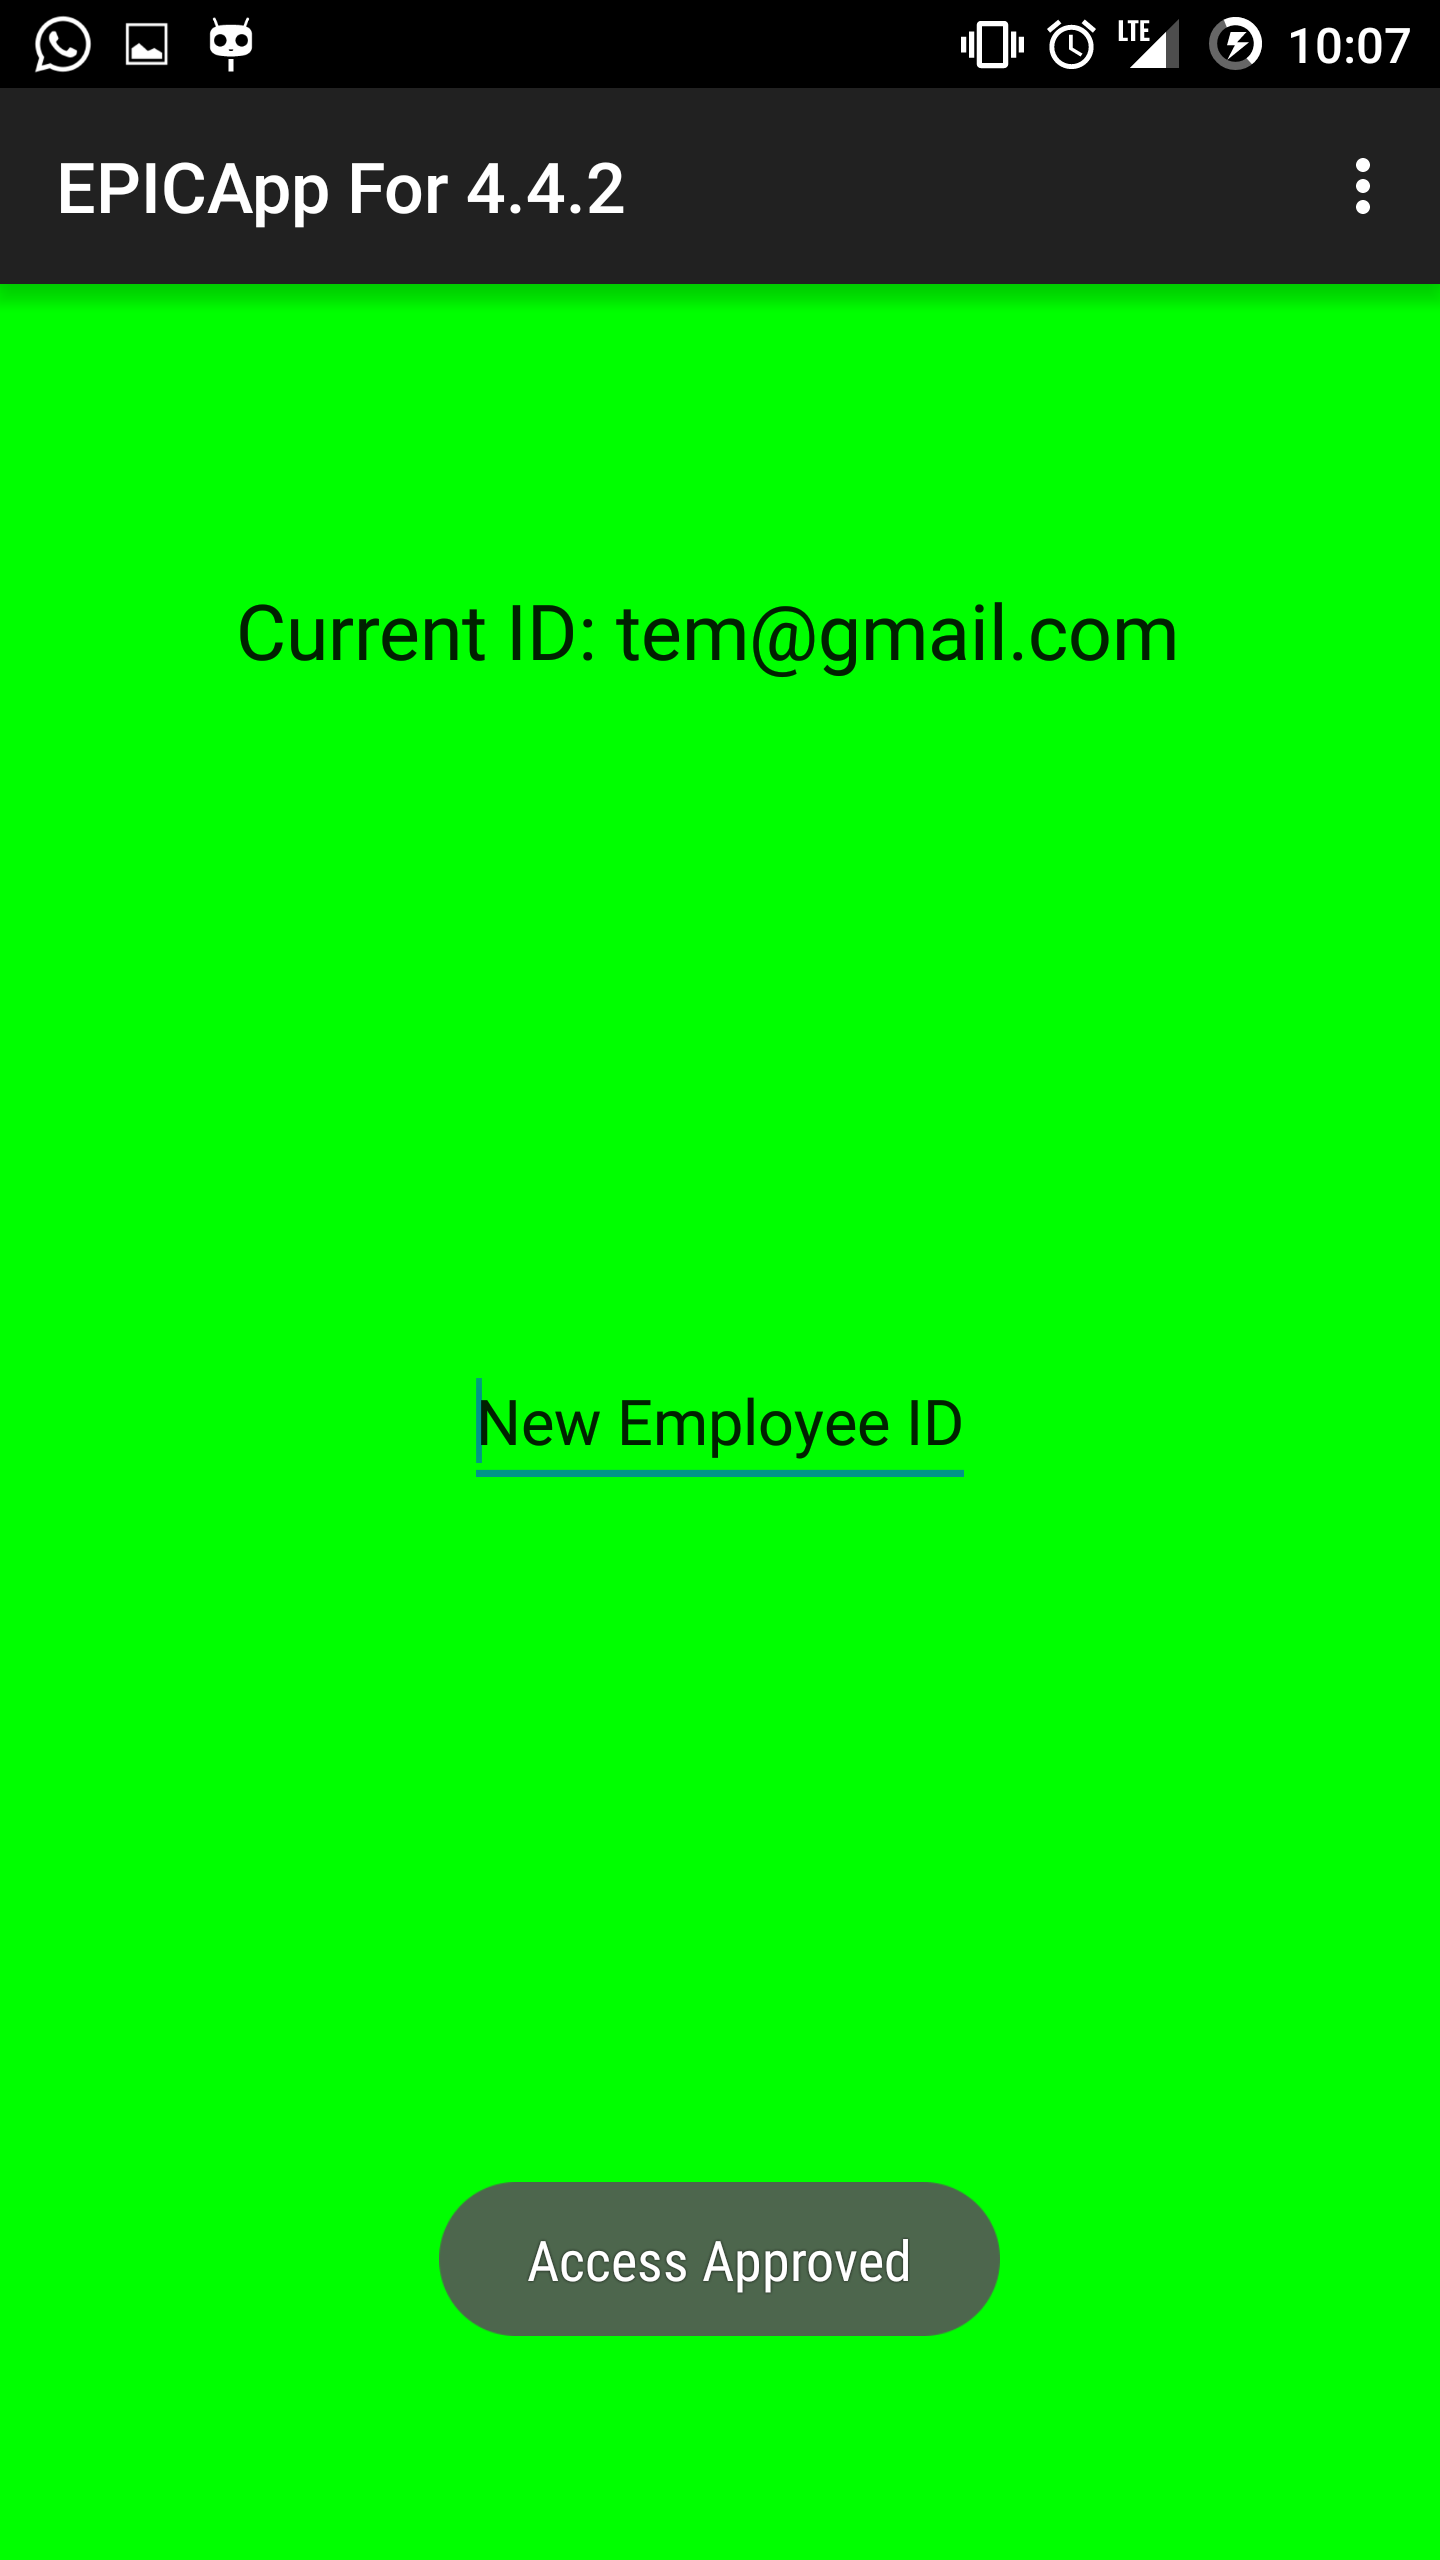
\includegraphics[height=6cm]{Approved}
                    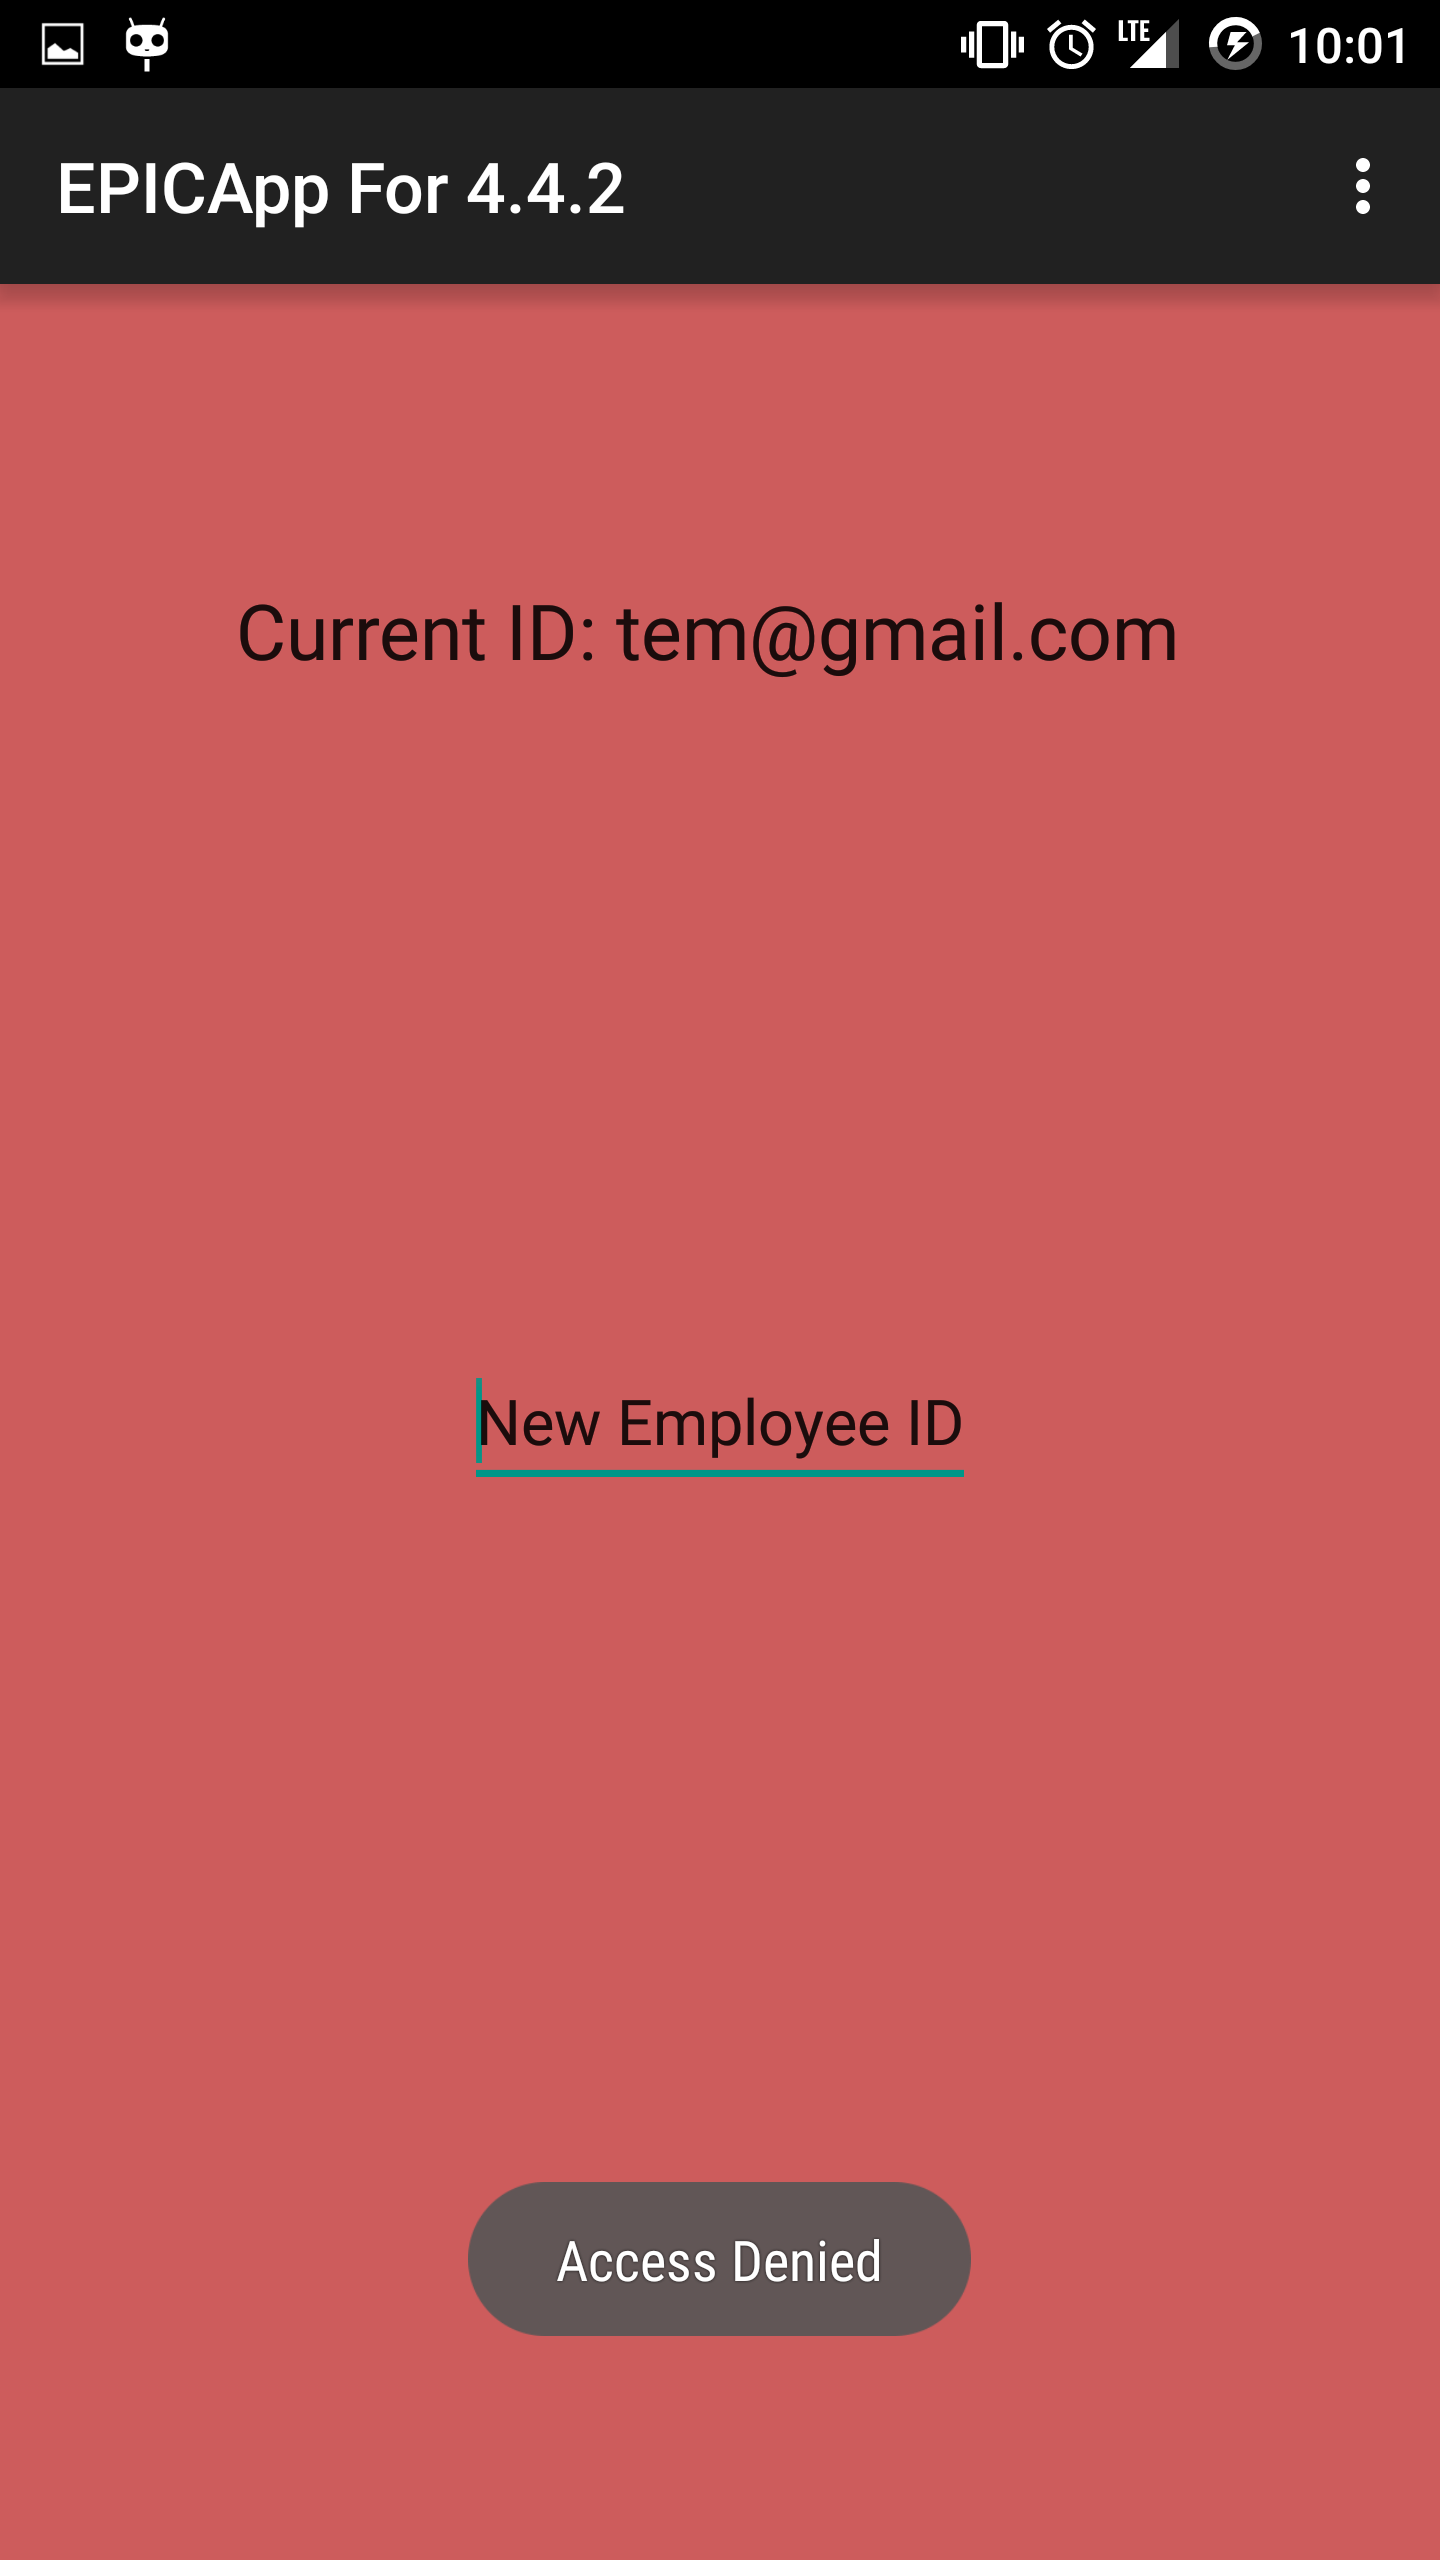
\includegraphics[height=6cm]{Denied}
                    \caption{Approved and denied screens}
                    \label{fig:my_label3}
                    \end{figure}}
                For green flash go to step 3 and for red flash go to step 4.
                \item{You have gained access to the door and may enter or leave the room. Entering will turn communication channels off and leaving will turn them back on.}
                \item{You have been denied access. Make sure you are at the correct meeting room and that you have been added to attend the meeting.}
            \end{enumerate}
        \item   To change users follow these steps:
            \begin{enumerate}
                \item{ Screen there is an edit box with the text \textit{New Employee ID} or your current ID. Click on it and type in the registered ID given to you and press the done or check mark key.
                    \begin{figure}[H]
                    \center
                    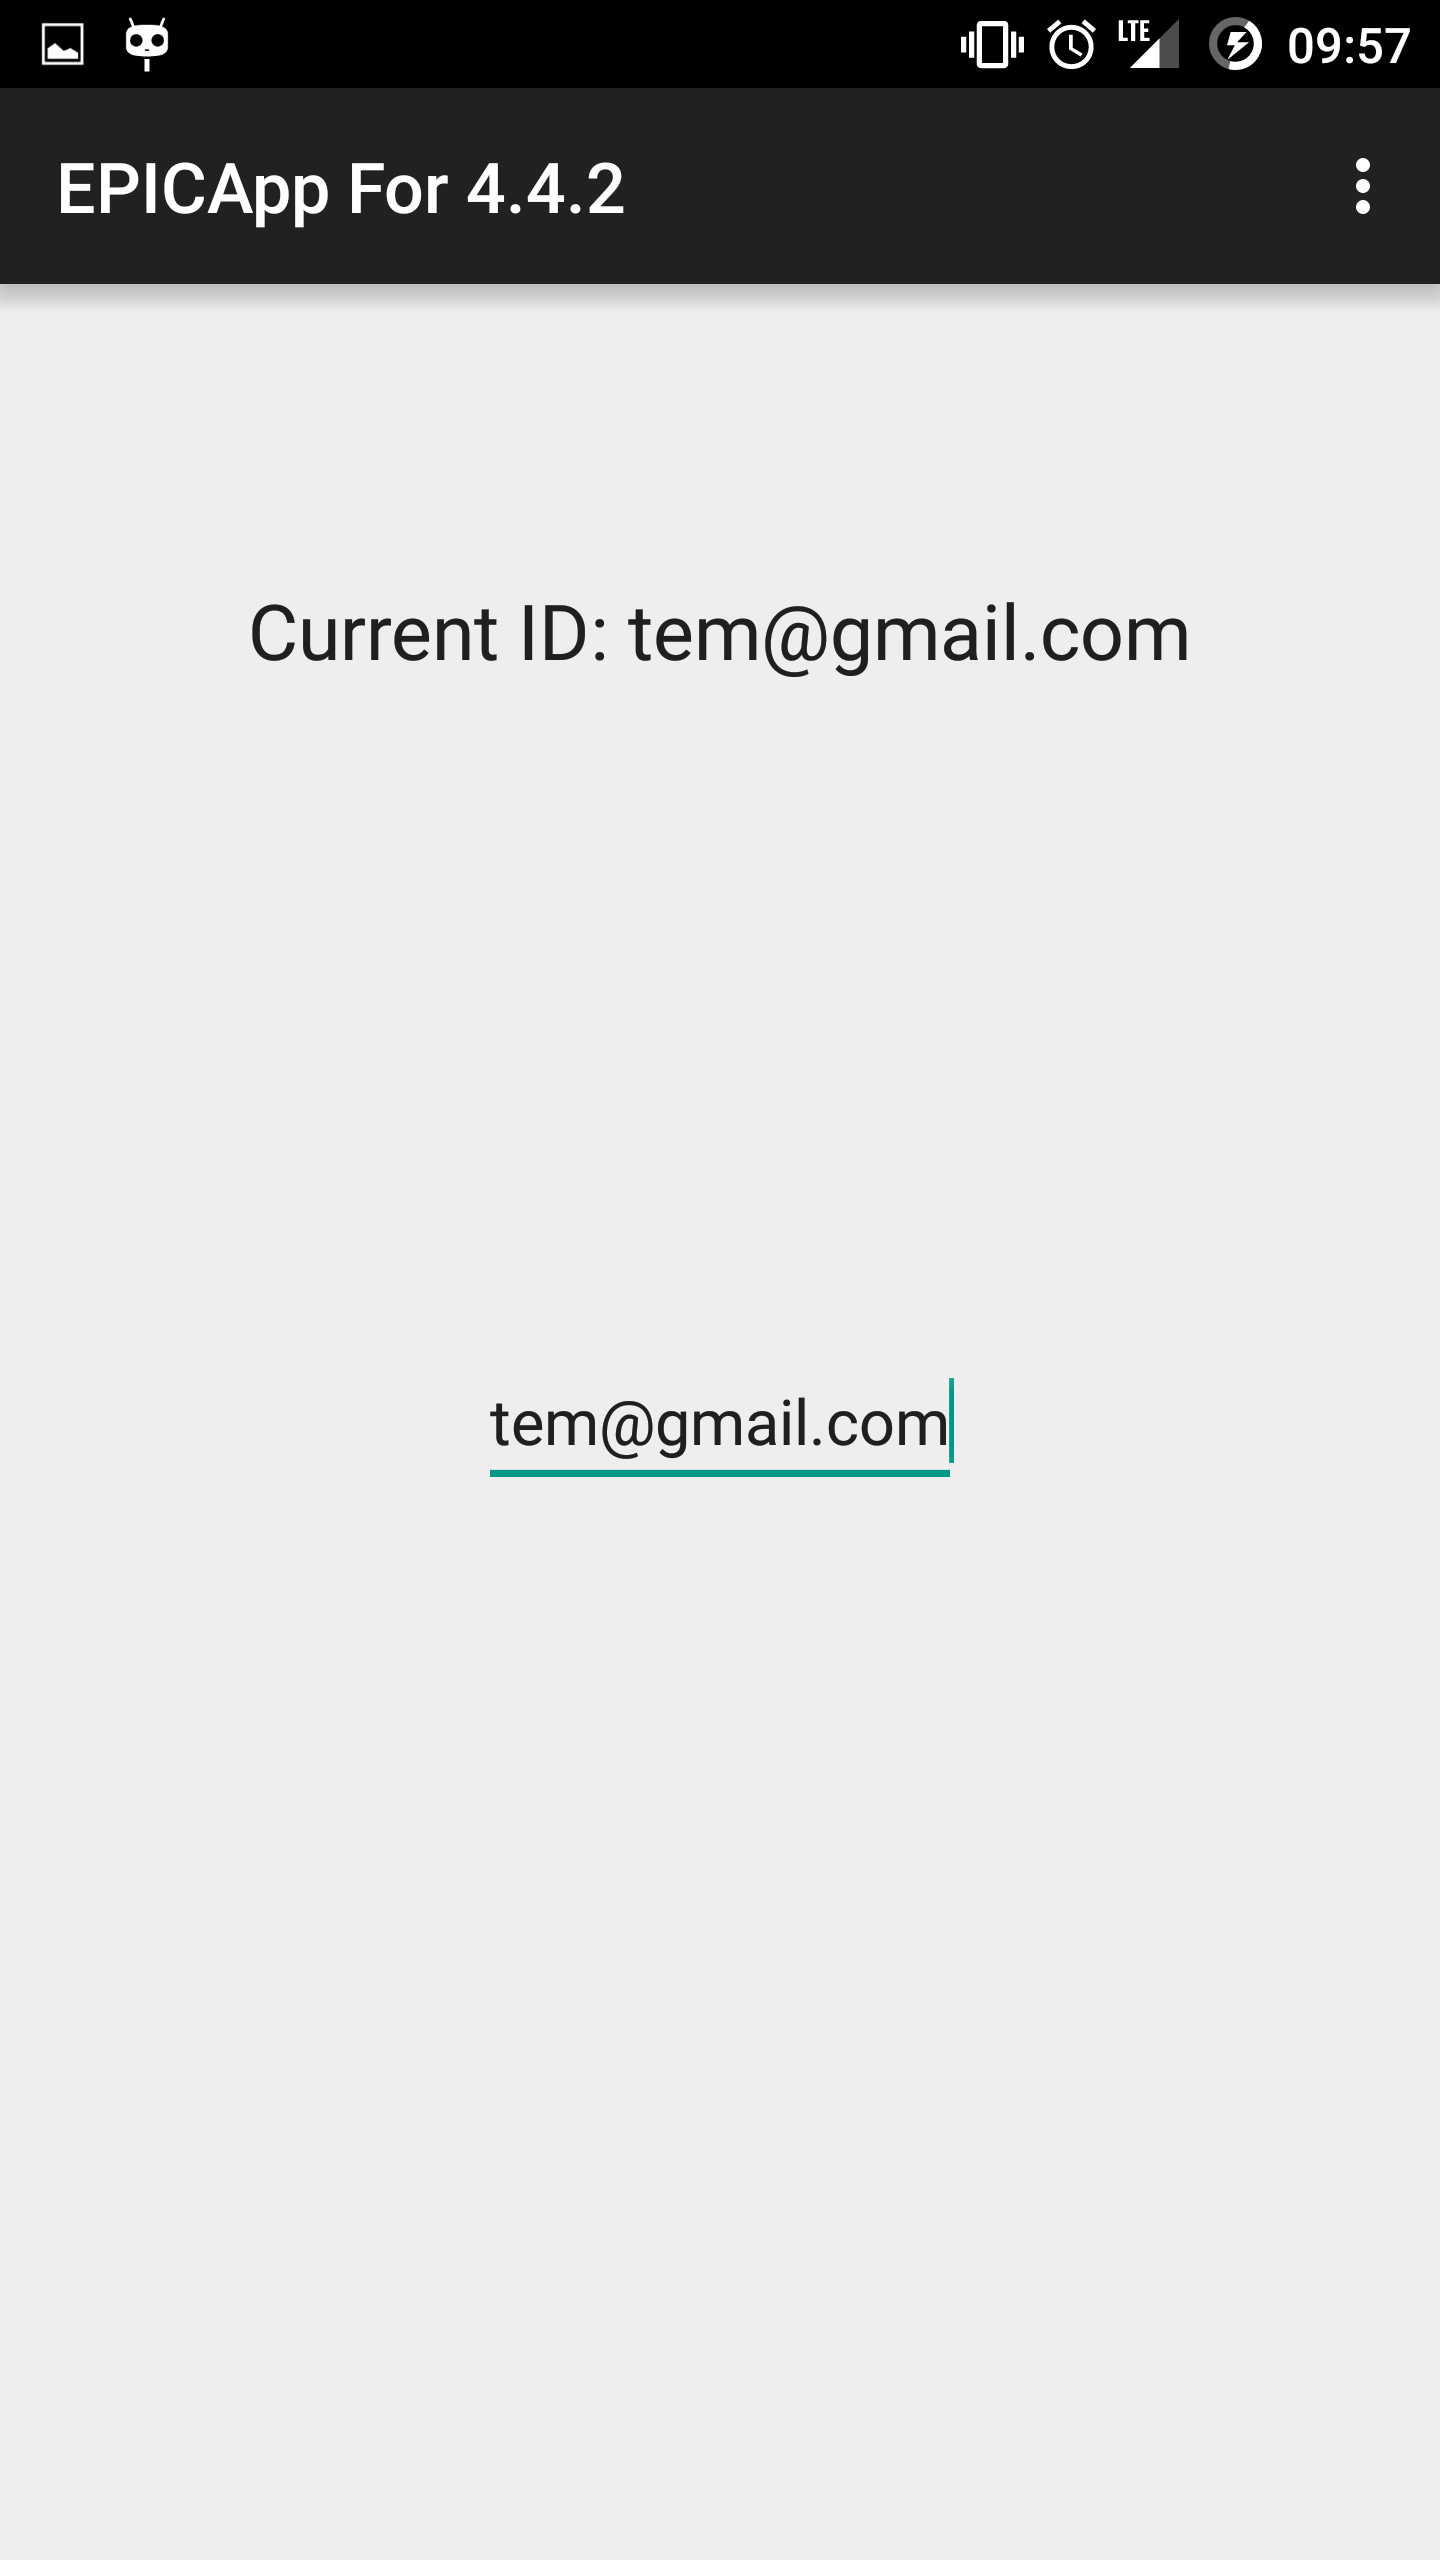
\includegraphics[height=6cm]{SecOpen}
                    \caption{Main Screen}
                    \label{fig:my_label4}
                    \end{figure}}
                \item You will notice the text at the top change to your ID that you typed in. This means that the application is now ready to be used to enter and leave the meeting room.
            \end{enumerate}
    \end{itemize}

\subsection{Node}
    If the Node is plugged in and functioning correctly, the lights should be Orange and Yellow strips running across. If this isn't the case, see the Troubleshooting section of this document.
    
    The Node has the following states:
    \begin{itemize}
       \item {\textbf{Ready and Waiting}: The lights running strips of yellow and orange.}
       \item {\textbf{Processing}: The lights have a blue bar counting up and a White light running back and forth.}
       \item {\textbf{Denied access by the server to the meeting}: All the lights are red.}
       \item {\textbf{Approved access by the server to the meeting}: All the lights are green.}
       \item {\textbf{Something went wrong}: All the lights are orange.}
       \end{itemize}
      Here is what you can do and when:
        \begin{itemize}
        \item In the ready and waiting state you can place your phone on the Node with the protection app open.
        \item In the processing state you must leave your phone on the node.
        \item When the lights have either turned Green, Red or Orange, you can remove your phone from the Node.
    \end{itemize}

\subsection{Website}
    \begin{itemize}
        \item If you want to register, open \url{http://projectepic.info/register} in your favourite web browser. Type your details in and click on the \textit{Register} button. After you have registered, you will automatically be logged in. It will look like this: 
        \begin{figure}[H]
                \centering
                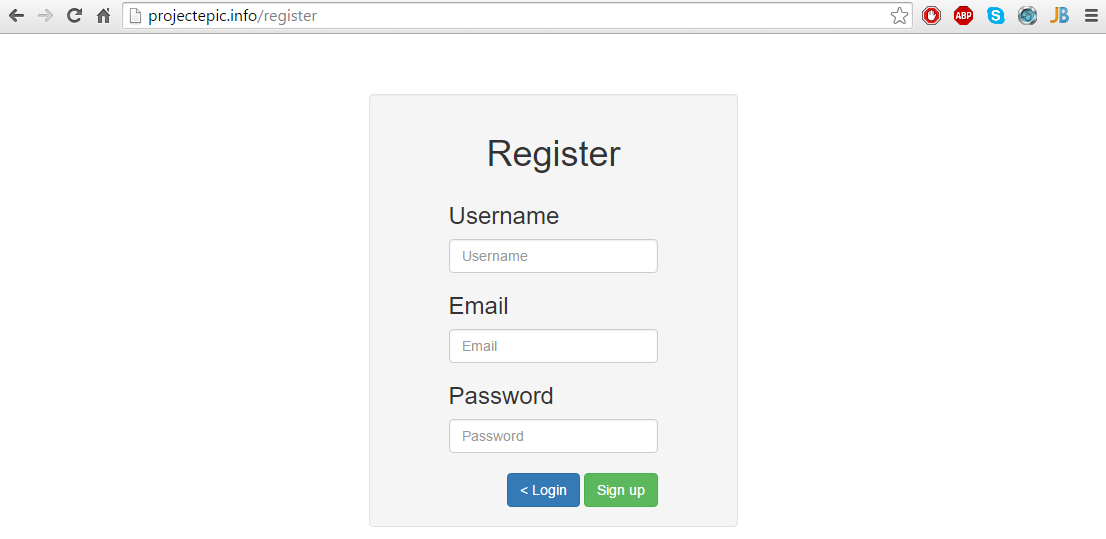
\includegraphics[width=10cm]{webPics/register}
                \caption{Website Register Page}
                \label{fig}
            \end{figure}       
        \item {If you have registered, you may log in at \url{http://projectepic.info}. Simply type in your details and then you may log in by pressing the \textit{Log in} button. You can also log in via Facebook. It will look like this: 
        \begin{figure}[H]
                \centering
                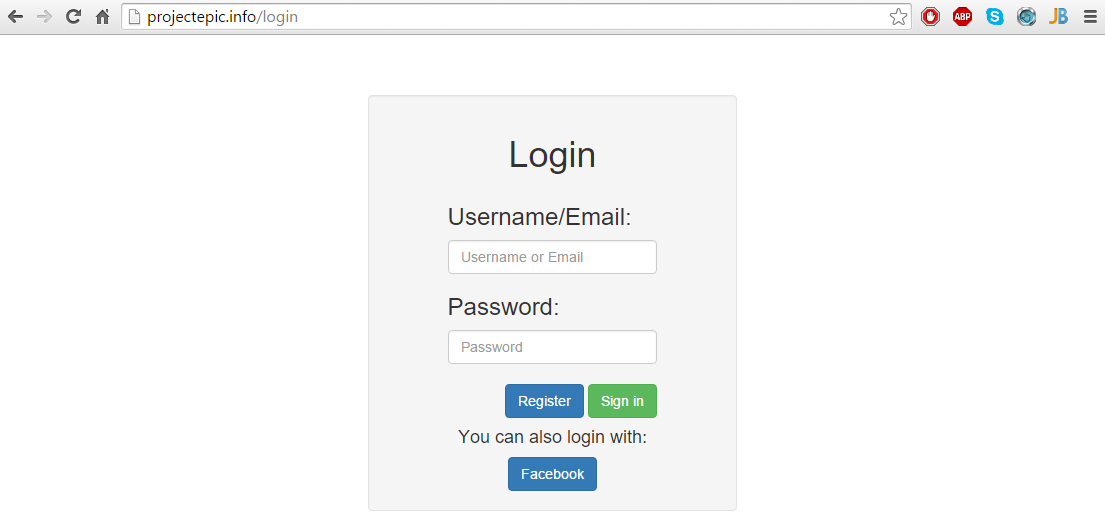
\includegraphics[width=10cm]{webPics/login}
                \caption{Website Login Page}
                \label{fig}
            \end{figure}}
        
        \item {To schedule a meeting you must redirect your browser to \url{http://projectepic.info/meetings}. You can then add another meeting by filling out the details. You can remove a meeting simply by clicking on the \textit{Remove} button next to the meeting details. 
        \begin{figure}[H]
                \centering
                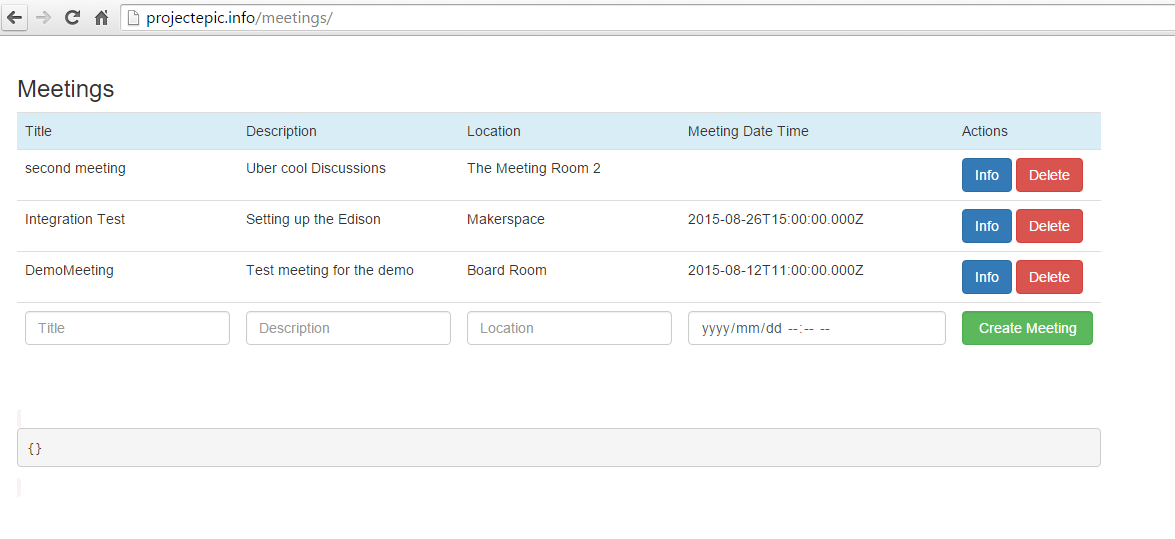
\includegraphics[width=10cm]{webPics/meetings}
                \caption{Website Meetings Page}
                \label{fig}
            \end{figure}}
            
            \item {If you wish to invite people to your meeting, click on the blue \textit{Info} button next to the meeting. The list of invitees will then appear to the right. To invite people, type in their details in the fields and click on the \textit{Invite} button. An invitation will then be send to them via email. You may also remove an invitee by clicking on the \textit{Remove} button next to their name. 
          \begin{figure}[H]
                \centering
                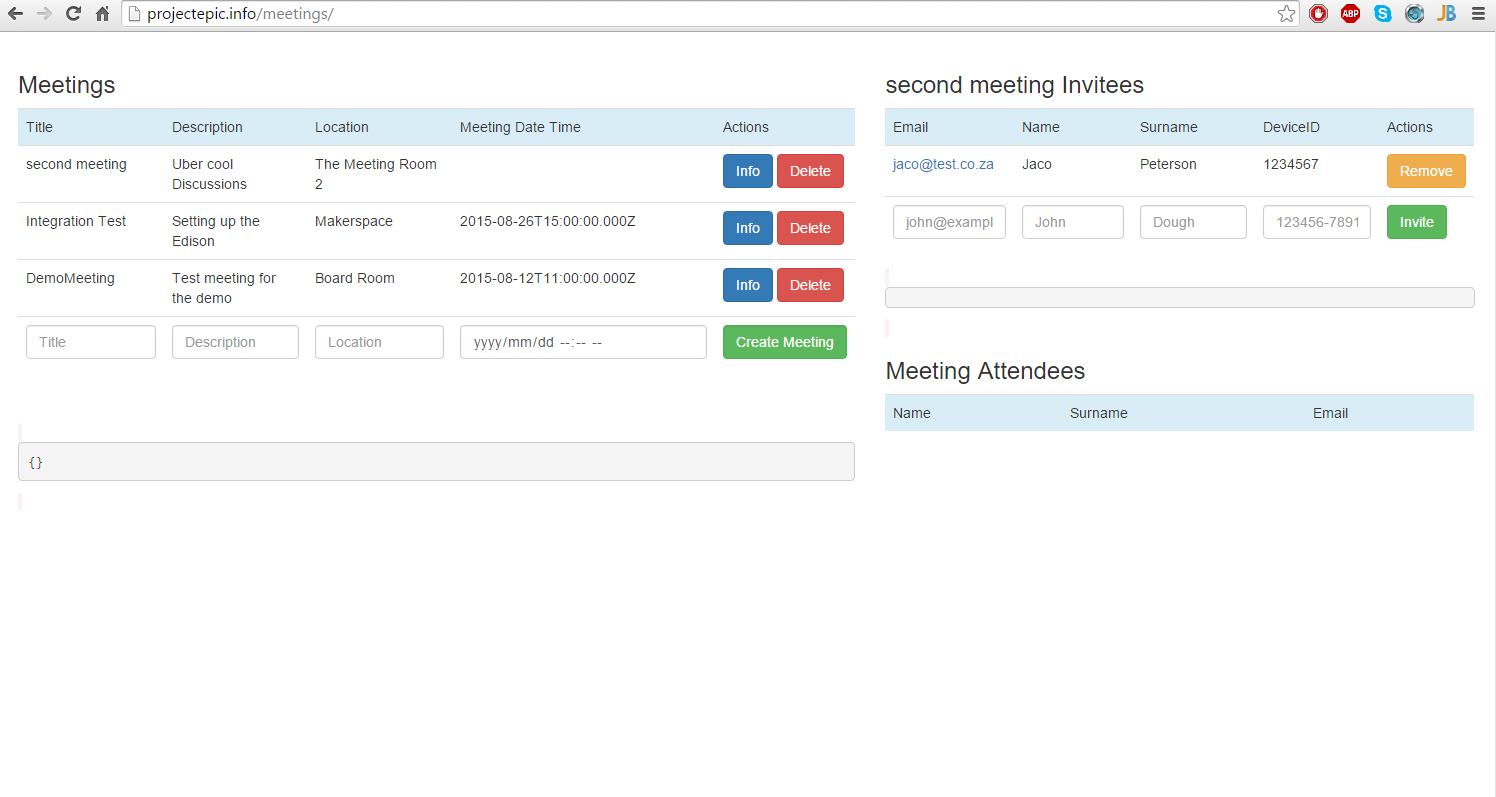
\includegraphics[width=10cm]{webPics/meetinginfo}
                \caption{Website Meeting Invites Page}
                \label{fig}
            \end{figure}}          
            

    \end{itemize}



\newpage
\section{Troubleshooting}
\subsection{Android Application}
\begin{itemize}
    \item If you cannot find the application on the store it means that you either do not have the correct Android Operating System(4.4), your device doesn't have NFC or your device doesn't support HCE(Host Card Emulation). Consult your device's manual.
    \item If the application is not scanning (changing colour), check that NFC is turned on.
    \item If you cannot access a room that you should have access to, make sure that you spelling of your employee ID is correct (the system is case sensitive). Also confirm that you have been added to the meeting.
\end{itemize}

\subsection{Node}
\begin{itemize}
    \item If the lights turn Orange after you scanned your phone, you can check the Server or Gateway for error codes.
    \item If the lights are off or frozen and the problem doesn't go away after a few seconds, you can either plug it out and in again or check what caused this on the Gateway.
\end{itemize}


\subsection{Website}
\begin{itemize}
    \item If the elements on the website overlap, adjust the size of the browser window.
    \item If the button doesn't work, wait patiently for the project to finish.
    \item If the server is not found, wait a few minutes and try again.
\end{itemize}



\end{document}
